\documentclass{report}

% packages
\usepackage[utf8]{inputenc}
%\usepackage[linesnumbered,lined,boxed,commentsnumbered]{algorithm2e}
\usepackage[ruled,vlined,noend,linesnumbered]{algorithm2e}
\usepackage{amsthm}
\usepackage{amsmath}
\usepackage{amssymb}
\usepackage{enumerate}
\usepackage{dsfont}
\usepackage{graphicx}
\usepackage[margin=1.4in]{geometry}

\usepackage{calrsfs}
\DeclareMathAlphabet{\pazocal}{OMS}{zplm}{m}{n}
\DeclareMathOperator*{\polylog}{polylog}

% definitions and commands
\newtheorem{theorem}{Theorem}[section]
\newtheorem{lemma}[theorem]{Lemma}
\newtheorem{conjecture}[theorem]{Conjecture}
\newtheorem{corollary}[theorem]{Corollary}
\newtheorem{proposition}[theorem]{Proposition}
\newtheorem{definition}[theorem]{Definition}

\newcommand{\norm}[1]{\left\lVert#1\right\rVert}

\title{- CS344 Discrete Mathematics Project - \\  Incremental Cycle Detection \& Topological Ordering}
\author{Martin Costa}
\date{October 2020}

\begin{document}

\chapter{The Recourse Problem}

\section{Problem Definition}

In this chapter I shall introduce a new variant of incremental topological ordering which I will be focusing on throughout the rest of this report; I shall refer to it as the \textit{recourse problem}. This problem is a combinatorial version of incremental topological ordering, where the objective is to design a high level algorithm for incremental topological ordering which minimizes a metric that we shall refer to as \textit{recourse}. I will then give descriptions of two simple high level algorithms that are currently candidates to solve an open problem on this topic.

Let $G=(V,E)$ be a DAG. Suppose we have an algorithm for incremental topological ordering, $\pazocal A$, which given an insertion sequence $\pazocal E \in \mathcal S_E$ maintains an ordering $\prec$ as the edges are inserted. We define a \textit{node movement} to be the operation of changing the position of a single node in the ordering, this can be thought of as removing any node and placing it back in at any position. Assume that the algorithm $\pazocal A$ can only affect the ordering by performing such node movements, we formalize the notion of \textit{recourse} as follows.

\begin{definition}[Recourse]
The \textit{recourse} of $u \in V$ caused by $\pazocal E_t$ during the run of $\pazocal A$ on $G$ with insertion sequence $\pazocal E$ starting with initial ordering $\prec$ is
\[ rec_u(\pazocal E, \prec)_t = \begin{cases} 
      1 & \textnormal{$\pazocal A$ moves $u$ while handling the insertion of $\pazocal E_t$}\\
      0 & otherwise \\
   \end{cases}
\]

The \textit{recourse} of $u$ created during the run of $\pazocal A$ on $G$ with insertion sequence $\pazocal E$ and initial ordering $\prec$ is $rec_u(\pazocal E, \prec) = \sum_{t=1}^m  rec_u(\pazocal E, \prec)_t$. The \textit{total recourse} created during the run of $\pazocal A$ on $G$ with insertion sequence $\pazocal E$ and initial ordering $\prec$ is $rec(\pazocal E, \prec) = \sum_{u \in V} rec_u(\pazocal E, \prec)$.
\end{definition}

\section{Why Recourse?}

This notion of recourse is quite a natural metric to consider for algorithms of this form. We can see that it gives us a lower bound on their runtime without having to consider any concrete implementations, since each swap will be performed individually by the algorithm by assumption. Hence if the worst case recourse of $\pazocal A$ is $\Omega(f(n))$ then the worst case runtime of $\pazocal A$ is also $\Omega(f(n))$.

However, the notion of recourse isn't only useful for algorithms that have this restricted form. Informally speaking, we can also see that given any incremental topological ordering algorithm, $\pazocal A$, if $\pazocal A$ can be modified to create an algorithm $\pazocal A^*$ that only affect the ordering with node movements such that $\pazocal A^*$ doesn't perform worse than $\pazocal A$, then $\pazocal A^*$ having a high recourse will give us that $\pazocal A$ will also have a high runtime. While this statement is quite informal and vague, it should give some intuition as to why recourse is a natural metric to consider in an attempt to simplify the problem. Even if it doesn't provide us with a formal reduction, it could give us some very useful insights while allowing us to work in a much simpler setting from a conceptual and technical perspective. Because we only need to worry about high level algorithms when considering recourse, trying to bound the recourse of an algorithm can be a much easier task than trying to bound the runtime directly, which will most likely require a more detailed concrete implementation of the algorithm.

As of now, there are currently no known algorithms that have been proven to have a \textit{worst case total recourse} or even an \textit{expected total recourse} of $\tilde {\pazocal O}(m)$ on all instances, i.e. algorithms that have worst case or expected polylogarthmic recourse per update/insertion on all graphs, and it is an open problem.\footnote{I use the notation $\pazocal{\tilde{O}}$ to hide poly-logarithmic factors, i.e. $\pazocal{\tilde{O}}(f(n))$ = $\pazocal O (f(n) \polylog f(n))$} In the following chapters I shall be giving many original frameworks and results relating to the recourse problem.

\section{The Simple Algorithms}

In this section I will introduce two very natural high level algorithms for incremental topological ordering. Before doing so, I will give a relevant definition to set the scene and make things a little easier.

\begin{definition}[Affected Region]
Suppose we are running some incremental topological ordering algorithm, and have a topological ordering of the current graph, $\prec$. If we insert some edge $e=(u,v)$ into the graph, then the \textbf{affected region} is the section of the ordering between $u$ and $v$, including $u$ and $v$. If a node is in the affected region we say it's an \textbf{affected node}.
\end{definition}

Many of the simplest algorithms for incremental topological ordering only rearrange nodes that are contained in the affected region after an insertion. This leads to a very natural class of algorithms that was first identified by Haeupler et al. [HKMST11] which they referred to as \textbf{local} algorithms and are formally defined as follows.

\begin{definition}[Local Algorithms]
Suppose we have some incremental topological ordering algorithm, $\pazocal A$, which maintains a topological ordering of the graph, $\prec$, as edges are inserted. Suppose we insert an edge $e=(u,v)$ into the graph, then $\pazocal A$ is \textbf{local} if
\begin{enumerate}
    \item $\pazocal A$ does not rearrange any nodes if $\prec$ is still a topological ordering for the updated graph
    \item $\pazocal A$ only rearranges the nodes in the affected region of $\prec$
\end{enumerate}
\end{definition}

While local algorithms may be simple and elegant, as we will see in later chapters, they also have limitations which makes it possible to design instances which can not be solved efficiently by \textit{any} local algorithm.

The two high level algorithms that I am about to describe, which I shall refer to as the \textit{simple} algorithms, are both local, so they are susceptible to such instances. However, in the next few chapters I shall be discussing variations of the recourse problem in different settings that may allow us to get past this issue, despite the limitations of local algorithms.

\subsection{A Remark on High Level Algorithms}

Because we only care about the recourse of these algorithms, we want high level descriptions of the algorithms that fully capture the effect they have on the ordering without worrying about their implementations, i.e. the data structures and mechanisms they use to achieve this effect. Because of this, I will be giving high level descriptions that will be intuitively clear and formal enough for our purposes but have no implicit or obvious associated concrete implementations.

\subsection{The One-Way Search Algorithm, $\pazocal A_1$}

The \textit{simple one-way search algorithm}, $\pazocal A_1$, is a local algorithm which can be split into 2 distinct phases: phase 1, a restricted forward-search, and phase 2, a sequence of node movements. Informally, after the insertion of an edge $(u,v)$, in phase 1 the algorithm performs a forward search of the affected region, starting from $u$, and creates a subsequence of the ordering with all the nodes it finds. In phase 2, the algorithm removes all the nodes in this subsequence from $\prec$ and places the whole subsequence back into $\prec$ just to the right of $u$.

\begin{algorithm}[H]\label{oneway}
    \SetAlgoLined
    \KwIn{DAG $G=(V,E)$, a topological ordering $\prec$ of $G$, and an edge $e = (u,v) \notin E$ such that $G \cup \{e\}$ is a DAG}
    \KwOut{a topological ordering $\prec^*$ of $G \cup \{e\}$}
    
    \If{$u \prec v$}{return $\prec$\;}
    
    $\triangleright$ let $(u_1,...,u_n)$ be the ordering $\prec$\;
    $\triangleright$ suppose $u = u_j$ and $v=u_i$ for some $1 \leq i < j \leq n$\;
    
    $S \leftarrow \varnothing$\;
    $k \leftarrow i$\;
    
    \While{$k \leq j$}{
        \If{$u_k \in reach_G(v)$}{
            $S.push(u_k)$\;
        }
        $k \leftarrow k+1$\;
    }
    
    \While{$S \neq \varnothing$}{
        $x \leftarrow S.pop()$\;
        move $x$ just to the right of $u$ in $\prec$\;
    }
    return $\prec$\;
    \caption{The Simple One-Way Search Algorithm, $\pazocal A_1$}
\end{algorithm}

\subsection{The Greedy Two-Way Search Algorithm, $\pazocal A_2$}

The \textit{simple greedy two-way search algorithm}, $\pazocal A_2$, is also a local algorithm that can be split into 2 distinct phases: phase 1, simultaneous restricted backwards and forwards searches, and phase 2, a sequence of node movements. Informally, after the insertion of an edge $(u,v)$, in phase 1 the algorithm performs two simultaneous forwards and backwards searches of the affected region, starting from $u$ and $v$ respectively, and creates two subsequences of the ordering with the nodes it finds during each search. The searches continue until they `meet each other in the middle'. In phase 2, the algorithm moves the nodes it found during the forward search to the right and the nodes it found during the backward search to the left in such a way that it restores the topological ordering.

\begin{algorithm}[H]\label{twoway}
    \SetAlgoLined
    \KwIn{DAG $G=(V,E)$, a topological ordering $\prec$ of $G$, and an edge $e = (u,v) \notin E$ such that $G \cup \{e\}$ is a DAG}
    \KwOut{a topological ordering $\prec^*$ of $G \cup \{e\}$}
    
    \If{$u \prec v$}{return $\prec$\;}
    
    $\triangleright$ let $(u_1,...,u_n)$ be the ordering $\prec$\;
    $\triangleright$ suppose $u = u_j$ and $v=u_i$ for some $1 \leq i < j \leq n$\;
    
    $S \leftarrow \varnothing, R \leftarrow \varnothing$\;
    $s \leftarrow i, r \leftarrow j$\;
    
    \While{$S.peek() \prec R.peek()$}{
        \If{$S.peek() \prec R.peek()$}{
            \While{$u_s \notin reach_G(v)$}{
                $s \leftarrow s+1$\;
            }
            $S.push(u_s)$\;
            $s \leftarrow s+1$\;
        }
        \If{$S.peek() \prec R.peek()$}{
            \While{$u_r \notin reach_G^{-1}(u)$}{
                $r \leftarrow r-1$\;
            }
            $R.push(u_r)$\;
            $r \leftarrow r-1$\;
        }
    }
    $x \leftarrow S.pop()$\;
    \While{$S \neq \varnothing$}{
        $y \leftarrow S.pop()$\;
        move $y$ just to the right of $x$ in $\prec$\;
        $x \leftarrow y$\;
    }
    $x \leftarrow R.pop()$\;
    \While{$R \neq \varnothing$}{
        $y \leftarrow R.pop()$\;
        move $y$ just to the left of $x$ in $\prec$\;
        $x \leftarrow y$\;
    }
    return $\prec$\;
    \caption{The Simple Greedy Two-Way Search Algorithm, $\pazocal A_2$}
\end{algorithm}

\subsection{A comparison of $\pazocal A_1$ and $\pazocal A_2$}

The algorithms $\pazocal A_1$ and $\pazocal A_2$ are very similar. The obvious difference is that $\pazocal A_1$ only performs one search while $\pazocal A_2$ performs two simultaneous searches. We say that $\pazocal A_2$ is a \textit{greedy} algorithm because it's strategy is roughly to try and minimize the number of node movements in a single update. Figure \ref{fig:simplesearch} gives a visual representation of $\pazocal A_1$ and $\pazocal A_2$ both handling the same edge insertion.

\begin{figure}[htp]
    \centering
    \centerline{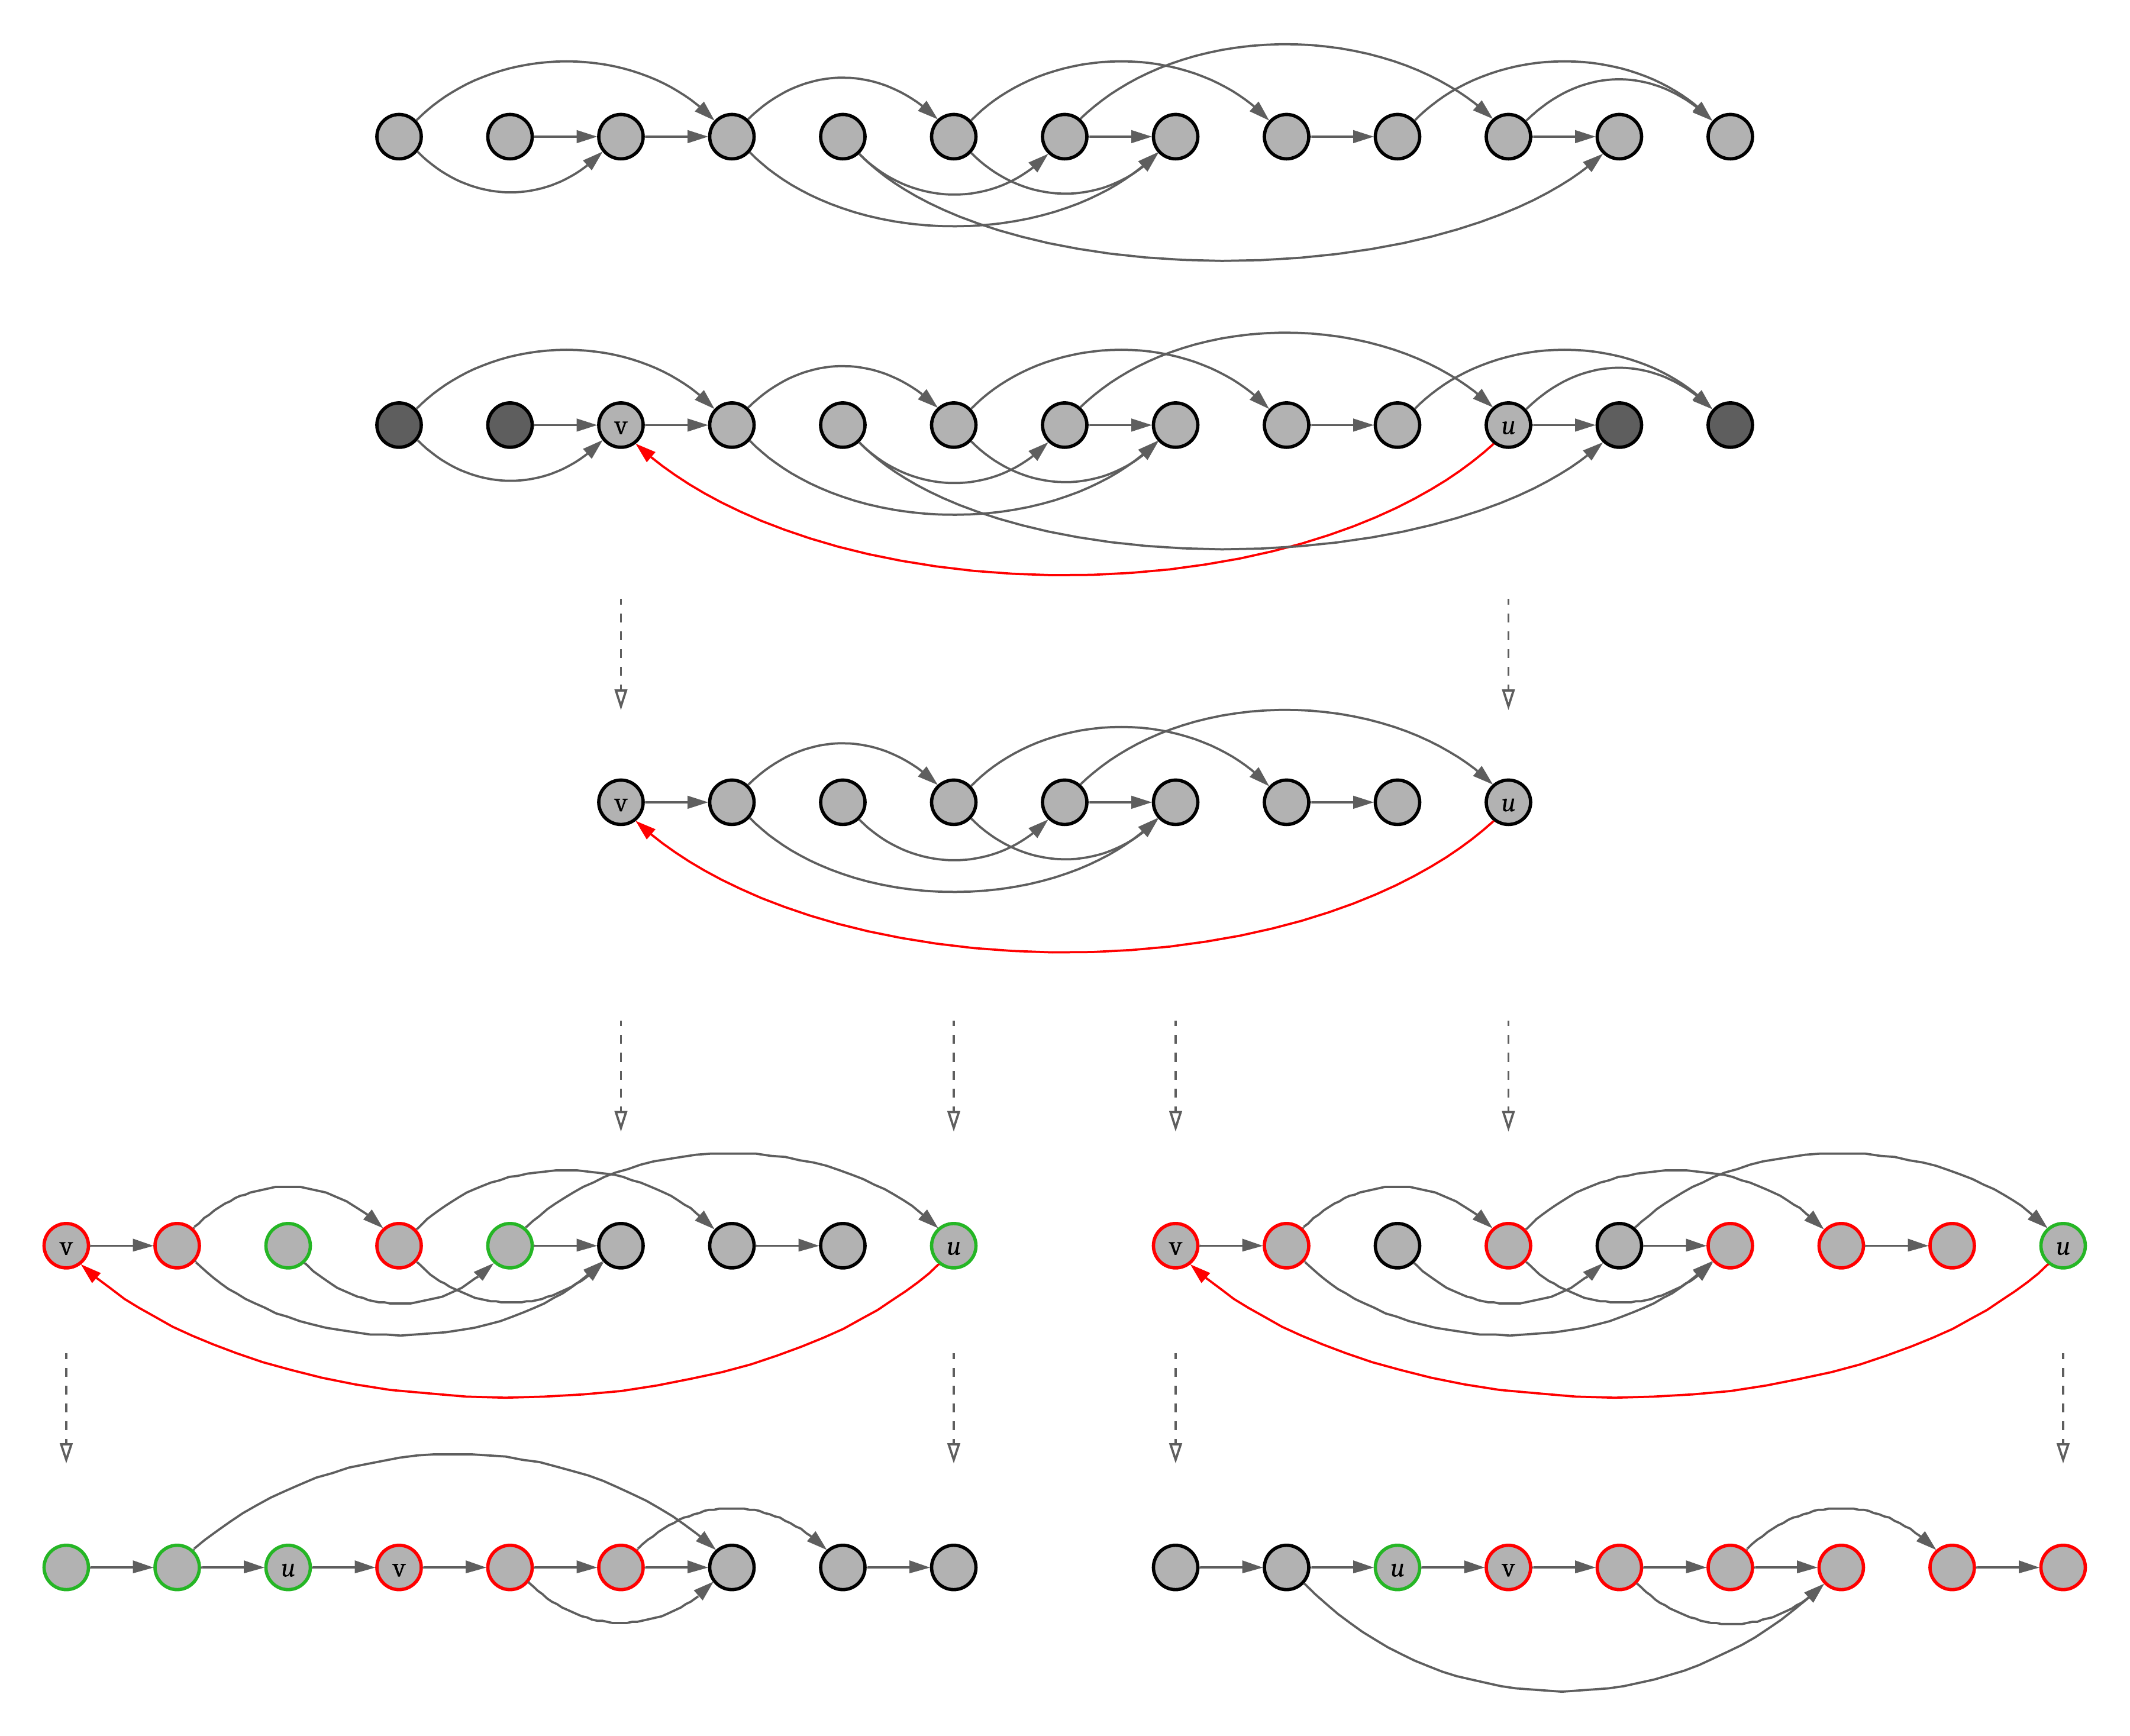
\includegraphics[width=16cm]{Simple Algos.png}}
    \caption{A comparison of the simple search algorithms, one-way search $\pazocal A_1$ (right), and greedy two-way search $\pazocal A_2$ (left), restoring the topological ordering after the insertion of $(u,v)$ by rearranging nodes in the affected region.}
    \label{fig:simplesearch}
\end{figure}

\section{Open Problems}

There are many open problems related to incremental cycle detection and topological ordering, including some related to the notion of recourse which I have just introduced. Most of these are mainly concerned with obtaining amortized polylogarithmic update times in certain settings, the most important (and also the hardest) of which is the question of whether there exists an algorithm for incremental cycle detection with a worst case or expected runtime of $\tilde{\pazocal O}(n)$ on all inputs. While this problem is notoriously hard and far outside the scope of this project, there are other open problems that are more accessible. Before covering these, I will briefly discuss the \textit{random-order model}, and it's potential relevance to incremental cycle detection and topological ordering.

\subsection{Random Order Arrival vs. Adversarial Arrival}

In the \textit{random-order model} for online algorithms, the input is chosen by an \textit{adversary} but is randomly permuted before being presented to the algorithm. This process of randomizing the order of the input can often weaken the power of the adversary.\footnote{Gupta el al. give a good survey of the random-order model and many examples in their paper [GS20]}

This model is very applicable in the context of incremental topological ordering; it's very natural to ask whether randomising the order of an insertion sequence before presenting it to some algorithm will provide us with improved algorithmic guarantees. My supervisor, Sayan Bhattacharya, has conjectured that there exists an incremental topological ordering algorithm that has low expected recourse per insertion for any graph under random-order arrival. More formally, we have the following conjecture.

\begin{conjecture}\label{mainconjecture}
Let $G=(V,E)$ be a DAG and $\prec \: \in \mathcal S_V$ any initial ordering of $G$, then there exists some incremental topological ordering algorithm such that it's recourse satisfies the following
\[ \mathbb E_{\pazocal E \in \mathcal S_E}[rec(\pazocal E, \prec)] = \tilde{\pazocal O}(m) \]
\end{conjecture}

In fact, he has conjectured that the algorithms $\pazocal A_1$ and $\pazocal A_2$ have low expected recourse \textit{per node} (not just per insertion) for any graph under random-order arrival. In contrast, note that insertion sequences leading to high recourse can easily be constructed for both of these algorithms under adversarial arrival. More formally, we have the following conjectures.

\begin{conjecture}\label{A1conjecture}
Let $G=(V,E)$ be a DAG and $\prec \: \in \mathcal S_V$ any initial ordering of $G$, then the recourse of the simple one-way search algorithm, $\pazocal A_1$, satisfies the following
\[ \mathbb E_{\pazocal E \in \mathcal S_E}[rec(\pazocal E, \prec)] = \tilde{\pazocal O}(n) \]
\end{conjecture}

\begin{conjecture}\label{A2conjecture}
Let $G=(V,E)$ be a DAG and $\prec \: \in \mathcal S_V$ any initial ordering of $G$, then the recourse of the simple greedy two-way search algorithm, $\pazocal A_2$, satisfies the following
\[ \mathbb E_{\pazocal E \in \mathcal S_E}[rec(\pazocal E, \prec)] = \tilde{\pazocal O}(n) \]
\end{conjecture}

Since for both of these algorithms we can assume that the input graphs are weakly connected (it can be shown that the effect of either algorithm on some node $u \in V(G)$ only depends on the structure of $G[reach_G(u) \cup reach^{-1}_G(u)]$, so we only have to consider graphs which are weakly connected), we can assume without loss of generality that $m=\Omega(n)$. Hence, Conjecture \ref{A1conjecture} and \ref{A2conjecture} both individually imply Conjecture \ref{mainconjecture}.

\subsection{Experimental Results}

Before I started thinking about these problems, I implemented the simple algorithms, $\pazocal A_1$ and $\pazocal A_2$, and tested them on many randomly generated graphs.\footnote{All the code for these implementations can be found at github.com/martin-costa/incremental-cycle-detection} All the data I collected supports both of these conjectures. Figure \ref{fig:recoursetests1} shows some of the data. I have not included the details of how I generated the DAGs or the insertion sequences since I want to focus on concrete results and not experimental data. However, I did try many different techniques and attained the same results each time. All of these tests can also be found in the repository referenced earlier.

\begin{figure}[htp]
    \centering
    \centerline{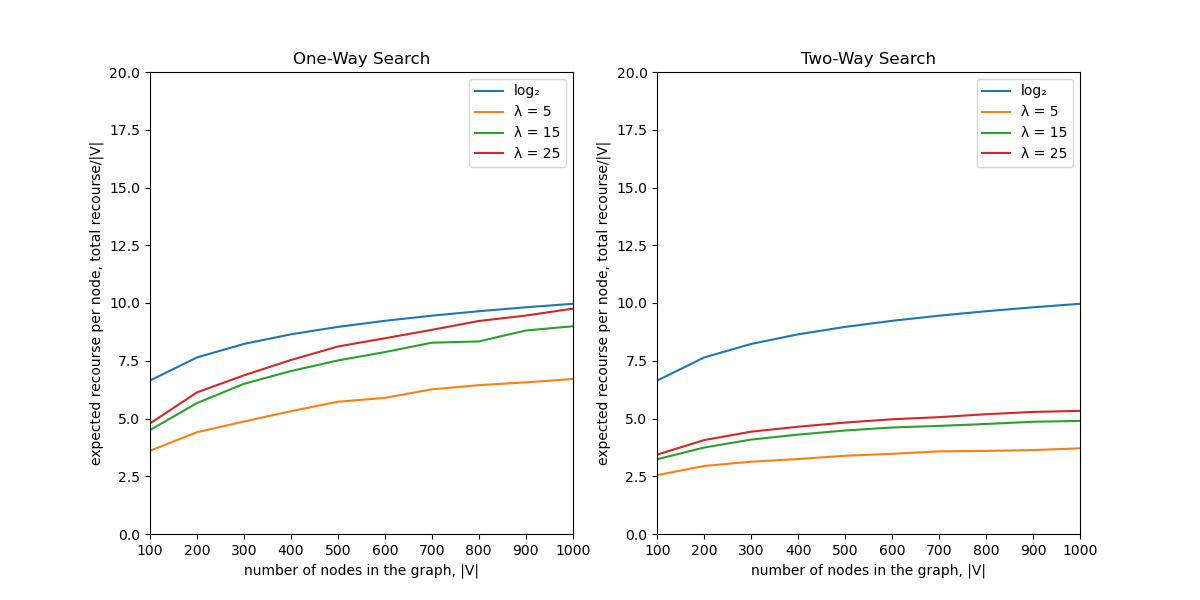
\includegraphics[width=18cm]{simple algo tests.png}}
    \caption{The curve $\lambda = k$ shows the average recourse per node (with respect to $\pazocal A_1$ on the left and $\pazocal A_2$ on the right) over many randomly generated insertion sequences of length exactly $\lambda n$ on randomly generated DAGs with $n$ nodes.}
    \label{fig:recoursetests1}
\end{figure}

\end{document}